\documentclass[tikz,border=5pt]{standalone}

\usepackage{tikz}
\usetikzlibrary{arrows.meta,automata,positioning,fit,backgrounds,calc}

\begin{document}

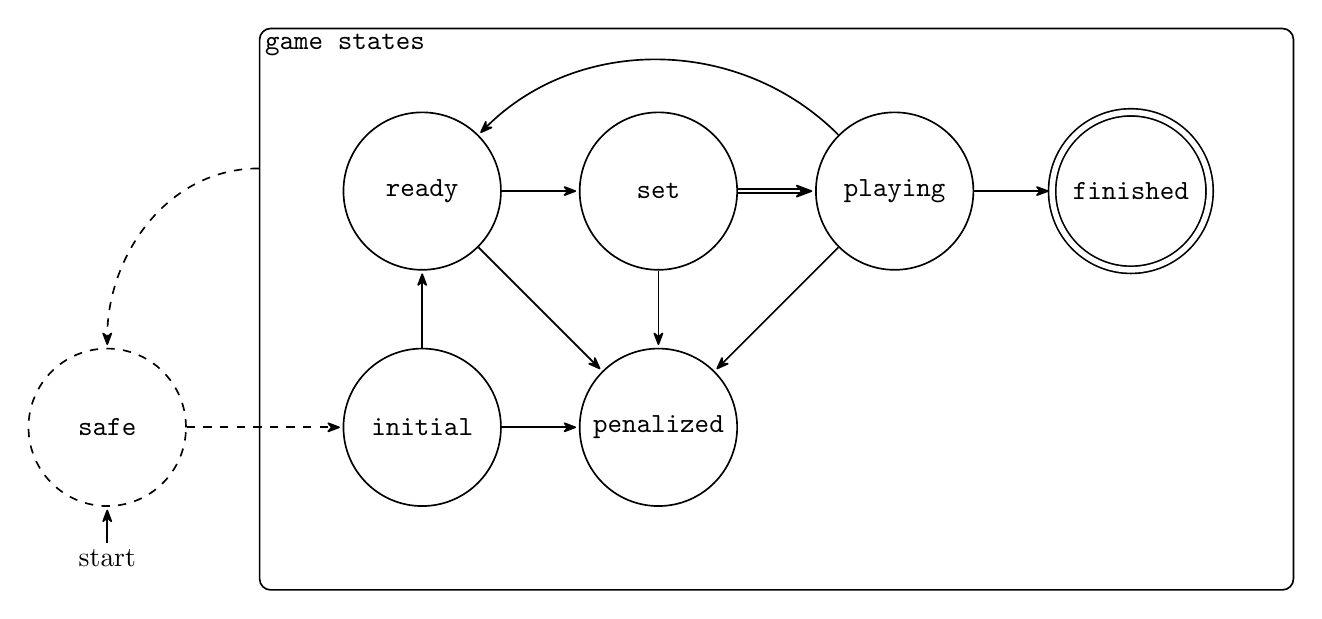
\begin{tikzpicture}[->,>={Stealth[round]},shorten >=1pt,
                    auto,node distance=3cm,on grid,semithick,
                    inner sep=2pt,bend angle=45]
    \tikzset{
      state/.style={
        circle,
        draw,
        minimum size=20mm,
        inner sep=0pt
      },
      superstate/.style={
        draw,
        rounded corners,
        %dashed,
        inner sep=30pt
      },
      accepting/.style={
        double,
        double distance=2pt
      }
    }
    
    % Game States
    \node [state] (initial)                      {\texttt{initial}};  
    \node [state] (ready)     [above=of initial] {\texttt{ready}};
    \node [state] (set)       [right=of ready]   {\texttt{set}};
    \node [state] (playing)   [right=of set]     {\texttt{playing}};
    \node [state, accepting] (finished)  [right=of playing] {\texttt{finished}};
    \node [state] (penalized) [right=of initial] {\texttt{penalized}};
    
    \node [state, initial, initial where=below, dashed] (safe)      [left=4cm of initial]  {\texttt{safe}};

    \node[superstate,
            fit=(initial)(ready)(set)(playing)(finished)(penalized),
            label={[anchor=north west]north west:\texttt{game states}}]
            (gamestates) {};

    % Game Transitions
    \path
        (initial)  edge (ready)
        (ready)    edge (set)
        (set)      edge [double, double distance=1pt] (playing)
        (playing)  edge (finished)
        (playing)  edge [bend right=45] (ready);
        
    % penalized
    \path
        (initial)  edge (penalized)
        (ready)    edge (penalized)
        (set)      edge (penalized)
        (playing)  edge (penalized);

    % Technical transitions
    \path
        (safe)     edge [dashed] (initial)
        ($(gamestates.west)!0.5!(gamestates.north west)$) edge [out=180, in=90, dashed] (safe);
\end{tikzpicture}

\end{document}